\documentclass[tikz]{standalone}
\usepackage{pgfplots}
\pgfplotsset{compat=1.18}
\definecolor{utnblue}{RGB}{0, 102, 204}

\begin{document}
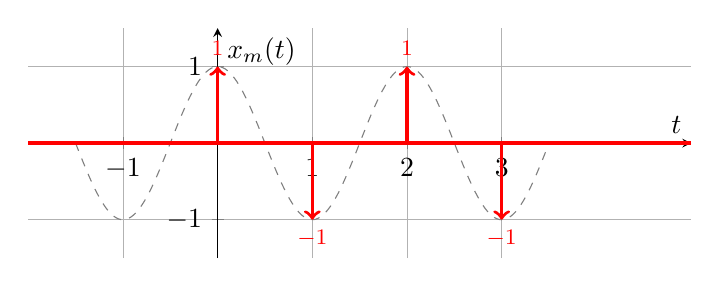
\begin{tikzpicture}
    \begin{axis}[
        width=10cm, height=4.5cm,
        axis lines=middle,
        xmin=-2, xmax=5, ymin=-1.5, ymax=1.5,
        xlabel={$t$}, ylabel={$x_m(t)$},
        grid=both,
        grid style={line width=.1pt, draw=gray!40},
        major grid style={line width=.2pt,draw=gray!60},
        xtick={-1,0,1,2,3},
        ytick={-1,0,1},
        samples=200,
        domain=-1.5:3.5,
    ]
    % Coseno base en gris punteado
    \addplot[gray, dashed, thin] {cos(deg(pi*x))};
    % Nivel cero (la señal vale 0 en t != k)
    \addplot[very thick, red] coordinates {(-2,0) (5,0)};
    % Impulsos de muestreo
    \draw[->,very thick, red] (axis cs:0,0) -- (axis cs:0,1) node[above, font=\footnotesize] {$1$};
    \draw[->,very thick, red] (axis cs:1,0) -- (axis cs:1,-1) node[below, font=\footnotesize] {$-1$};
    \draw[->,very thick, red] (axis cs:2,0) -- (axis cs:2,1) node[above, font=\footnotesize] {$1$};
    \draw[->,very thick, red] (axis cs:3,0) -- (axis cs:3,-1) node[below, font=\footnotesize] {$-1$};
    \end{axis}
\end{tikzpicture}
\end{document}
